% @(#) $Id$

\section{Introduction}

%BEGINHTML <<this keyword marks parts of text to extract for HTML page>>
Mapyrus is software for
creating plots of points, lines, polygons and labels 
to PostScript (high resolution, up to A0 paper size),
Portable Document Format (PDF) and web image output formats.

Mapyrus is freely-available and is implemented entirely in Java,
using Java's platform independence,
2D Graphics, JDBC and multi-threading capabilities.

The software combines the following four features.

\begin{enumerate}
\item

A Logo or turtle graphics program.
%ENDHTML

An imaginary pen is moved around a page,
creating shapes that are drawn into an image file.
Reusable routines are built up using a BASIC-like language.
Branching and looping constructs enable complex shapes, symbols and patterns
to be be defined.  See Figure \ref{turtle}.

\begin{figure}[htb]

\includegraphics{turtle1.eps}
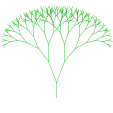
\includegraphics{turtle2.eps}

\includegraphics{turtle3.eps}
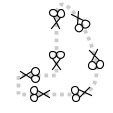
\includegraphics{turtle4.eps}
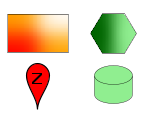
\includegraphics{turtle5.eps}
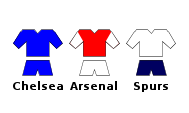
\includegraphics{turtle6.eps}
\caption{Shapes, Symbols And Patterns}
\label{turtle}
\end{figure}

%BEGINHTML
\item

Reading and displaying of geographic information
systems (GIS) datasets, text files, or tables held in a relational database
(including spatial databases such as PostGIS).
Drawing routines are applied to geographic data to produce annotated and
symbolized maps and graphs.  Attributes of the geographic data control
the color, size, annotation and other characteristics of the
appearance of the geographic data.
Scalebars, legends, coordinate grids and north arrows are also available.
%ENDHTML
See Figures \ref{mapview1}, \ref{mapview3}, \ref{mapview2} and
\ref{mapview4}.

\begin{figure}
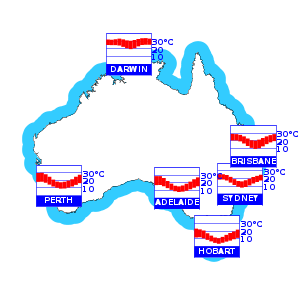
\includegraphics{mapview1.eps}
\caption[Average Monthly Temperatures]{Average Monthly Temperatures of Australian Cities (degrees Celsius)}
\label{mapview1}
\end{figure}

\begin{figure}
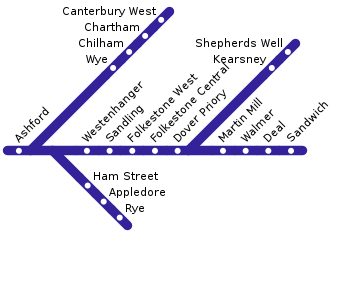
\includegraphics{mapview3.eps}
\caption{Strip Map of Railways Lines in East Kent}
\label{mapview3}
\end{figure}

\begin{figure}
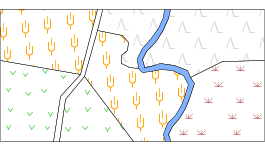
\includegraphics{mapview2.eps}
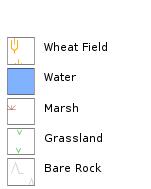
\includegraphics{mapview2legend.eps}
\vspace{1pt}
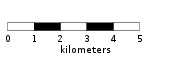
\includegraphics{mapview2scalebar.eps}
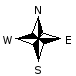
\includegraphics{mapview2north.eps}
\caption{Vegetation Classes}
\label{mapview2}
\end{figure}

\begin{figure}
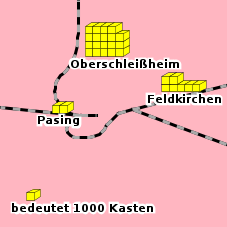
\includegraphics{mapview4.eps}
\caption{Inventory Levels at Warehouses}
\label{mapview4}
\end{figure}

%BEGINHTML

\item
Integration with the freely-available
\textit{Java Topology Suite} from Vivid Solutions
(\texttt{www.vividsolutions.com}).
This library provides geometric algorithms
such as buffering and polygon intersection.

\item
Flexibility.  Running in one of three ways.

\begin{enumerate}
\item
As a stand-alone program for integration into
scripts and batch tasks  (suitable for generating a one-off
map or a series of similar maps from a template
showing different areas, or using different criteria for each map).

\item
As a self-contained web server providing HTML pages, map and
graph images and text reports to a web-based application.

\item
As a Java API embedded in a Java application.
\end{enumerate}

\end{enumerate}

%ENDHTML

Please note that:

\begin{itemize}

\item
Mapyrus has no graphical user interface.
Commands are read from a text file prepared by the user.

\item
Mapyrus cannot display three dimensional data and has nothing to do
with 3D.

\item
Mapyrus does not include a library of ready-to-use symbols and patterns.
Users must define their own, using examples in this manual as a basis.
However, a large number of free icons
and TrueType format fonts found on the internet
defining shapes for animals, arrows and pointers, road signs, etc. are
available for use in Mapyrus.

\item
Mapyrus cannot reproject coordinate values in geographic data from
one projection to another.  However, this functionality
is available in spatial databases.
\end{itemize}

